% \documentclass{twocolumn,jsarticle}

\documentclass[twocolumn,10pt]{jarticle}

\setlength{\headheight}{0mm}
\setlength{\headsep}{0mm}
\setlength{\columnsep}{2zw} 

\usepackage[dvipdfmx]{graphicx}

\pagestyle{empty}


\title{交通システムとIoT}
\author{増井俊之 \\ 慶應義塾大学 環境情報学部}
\date{2019年3月29日}
\begin{document}
\maketitle

\thispagestyle{empty}

\abstract{
  電車やバスや自動車などの交通システムは
  長年にわたって現代社会に不可欠なインフラとなっている。
  また、パソコンやスマホのようなコンピュータや様々なセンサが
  ネットに接続されたIoT環境も社会のインフラとなりつつあるが、
  両インフラを統合的に活用するシステムはまだまだ発展途上である。
  交通システムとIoTを融合したシステムやサービスの可能性について考察する。
}

\section{はじめに}
  
ここ何年か「IoT」という単語がバズワードになっていたが、
最近はこの単語を聞く機会が減ってきた気がする。
あらゆる場所のセンサがインターネットに接続されることによって
世の中が激しく便利になることが期待されたのだろうが、
革新的な応用が充分開発されていないのかもしれない。

情報処理学会の学会誌「情報処理\footnote{
  \textsf{https://www.ipsj.or.jp/magazine/magazine.html}
}」では2019年初頭にしてIoT特集が組まれている。
2019年2月号の「社会を変えるIoT」という特集では
近年のIoT応用例が紹介されていたが、
水産業のために海の状況をモニタするシステム、
ノリ養殖支援システム、
養豚支援システムのような第一次産業での利用が最も多く、
その次に多いものが介護現場支援や子ども見守りシステムのような
弱者支援システムであった。
また、2019年3月号は「水産業におけるIoT」という特集で、
水産クラウド、
スマート水産データベース、
定置網での魚種判別、
赤潮監視システム
などが紹介されていた。

無線接続された沢山のセンサとコンピュータを実世界に配置して活用する技術は
従来は「センサネットワーク」と呼ばれることが多かった。
前述のような一次産業的な応用において
センサネットワーク技術が重要であることは間違いないが、
センサネットワークをベースとした新しいサービスは
あまり出現していないようである。
せっかく沢山のセンサやコンピュータが身の回りに沢山存在するのだから、
人間と一緒にセンサやコンピュータが移動したり、
人間とコンピュータとのインタラクションも利用できるような、
もっと面白い\textbf{アクティブなIoT}システムが
広まってほしいものである。

アクティブなIoTとは以下のような特徴をもつものである。

\begin{itemize}
  \setlength{\itemsep}{0cm} % 項目間  
  \item センサやコンピュータが人間と一緒に動く
  \item 人間のアクションや状態がIoT情報になる
  \item センサ情報にもとづいて人間がコンピュータを操作する
  \item 人間間のコミュニケーションに利用する
  \item 人間もセンサの区別をあまり行なわない
  \item 動き回る人間がセンサとして働く
  \item 人間がアクチュエータとして行動することもありうる
\end{itemize}

\section{交通系IoT}
  
電車やバスなどの公共交通機関は実用的で大規模な動的IoTを構築しやすい環境だといえる。
移動しまくる
電車とは限らない
自転車サーバ
数が膨大
電車はすごい数のセンサの運搬器である
なのに全然使われていない
普通の人間活動そのままでよい
人間と紐づけ
いろんな人間が移動しまくる
センサを持った人間が歩きまわる
人間がアクティブに何かをタッチする
人間をセンサにする話
HASC

交通系IoTには巨大な可能性があるが、現在のところは広く
すごい応用があるはずだがまだみつかっていないのだろう
情報の共有 /コミュニケーションへの利用
すいてる車輌/トイレ
遅れ情報の共有
トラブルの共有
自分情報の記録
どこに行ったか
日記になる

次のバスや電車がいつ来るのか? どれぐらい混んでいるのか?
というのはとても重要な情報であるにもかかわらず、
2019年になっても充分な情報がユーザに伝わっていない。


車輛内のセンサやGPSを利用すれば
現在位置や混雑状況は簡単に計測できるし、
それをネット上に公開することも簡単なのにもかかわらず、
こういうサービスが提供されていないのは不思議なことである。
予算や開発の手間といった問題はあるのかもしれませんが、
ーザを満足させるためのインタフェースの工夫が足りないと断言してしまっても良いでしょう。

電車やバスとはこういうものだから多少の不便は仕方がない」と思いこんでいる人が多いため、
IoT技術が実生活の改善に反映されていないのだと思われます。
  
自動改札の導入で磁気切符が主流になったり 交通系RFIDカードが導入された
りといった変化は記憶に新しいところですし、 トイレやエスカレータやエキ
ナカなどは昔に比べると激しく改善されてきていますが、 基本的な駅や電車
の使い方は100年以上あまり変わっていないようです。

寺田寅彦は、1947年の「電車の混雑について」という随筆\footnote{
  \small{\textsf{https://www.aozora.gr.jp/cards/000042/files/2449\_11267.html}}
}

で、すいた電車に乗るためのコツを述べています。

``必ずすいた電車に乗るために採るべき方法はきわめて平凡で簡単である。それはすいた電車の来るまで、気長く待つという方法である。''

  しばらく待った後に来る電車は混雑しているものであり、 客が一斉にそれに乗ろうとするとその電車はさらに混むはずですから、 混んだ電車はやり過ごして次の電車を待つのが得策だということです。 これは昔の東京の市電の話であり、時刻表通りに正確に運行される電車では状況は異なるかもしれませんが、 現代のバスの状況は似たようなものでしょう。 昔から電車の混雑には悩んできたということでしょう。
  寺田寅彦の時代とは異なり、現在はインターネットやセンサを自由に使えますから、 電車やバスの混雑具合や運行状況の情報は苦労なく取得して共有できるはずです。 あらゆるバスや電車がこういう情報を公開していれば混雑も緩和される可能性があります。

  \begin{figure}[htbp]
    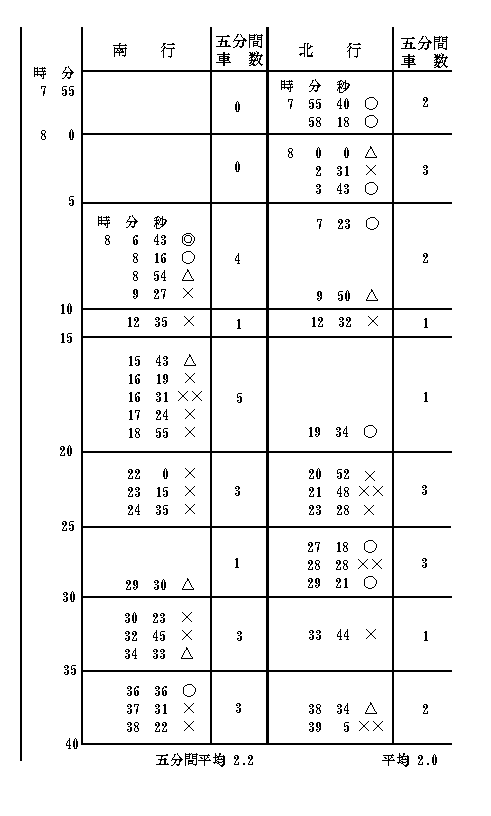
\includegraphics[clip,width=7.0cm]{./terada.png}
  \end{figure}

\paragraph{席を確保する}
  
  混んだ電車でも首尾良く座れれば辛くありません。 席が空いてなくても、座っている人が降りる駅がわかれば、 その人の前で席が空くのを待つことができます。 「靴を見ればだいたいどの駅で降りるかわかる」と豪語する人の話を聞いて驚いたことがありますが、 そういう超能力が無くてもセンサ技術を利用すれば降りる駅を判定できる可能性があります。
  お茶の水女子大学の笹川真奈氏は、 2014年の 未踏IT人材発掘・育成事業 に 「電車で効率よく座るための支援アプリケーションの提案と実装」というシステムを提案して 採択され、 それにもとづいた卒業論文を書きました。 このシステムでは、 乗客が持っているスマホなどのBluetooth信号を計測してデータベース記録することにより、 スマホを持つ人がどの駅で乗ったり降りたりするかを予測して降りそうな人を捜すようになっています。
  このようなデータベースを構築するのは大変でしょうし、 プライバシの懸念など様々な問題はありますが、 センサやネット情報を駆使することにより 電車で快適に過ごす可能性があることを示した意義は大きいと思います。 最新技術を駆使すれば、 靴や服装から降りる駅を判定するといったこともできるようになるのかもしれません。

\paragraph{乗り換え情報など}
  
  どの電車に乗れば早く目的地につくのか、 どう歩けばうまく乗り換えられるのか、 といった情報は重要ですが、 このような情報を得ることは現在でも簡単ではありません。 乗換案内のようなサービスを使えば こういった情報を知ることはできますが、 電車の運行状況や混雑状況も考えて電車を選ぶことはできません。
  スマホの乗換案内アプリなどで検索を行なった場合、 スマホは自分の予定を知っていることになりますから、 電車の運行状況や混雑状況、駅の構造などをもとにして 「右の階段を昇って4番線に移動」のように 最適な行動を提案することも可能なはずですが、 そういう情報は普通は提供されていないので 案内表示などを見て考えて行動する必要があります。 駅のサイネージに遅延などの運行状況を表示する努力は進んでいるようですが、 乗客がそれを注意して見て理解して最適な行動を考えなければならないようでは まだまだだといえるでしょう。

  電車に間に合うように行動するための 駅.Locky という画期的なアプリケーションがあります。 電車の時刻表はどこにでもありますが、 ある電車に乗れるかどうかを調べるためには 現在時刻、時刻表、自分の位置を考えて かなり頭を使わなければなりません。 駅.Lockyでは、 現在時刻や時刻表について調べなくても 「次の電車まで何分あるか」という情報だけを簡単に見ることができるので、 ユーザの負担はとても軽くなります。 電車に間に合うか調べるためには時刻表を見なければならないと私も思い込んでいましたが、 全く異なる解法を提示しているところに感心したものです。

  情報を提示/通知する

  ドアの上の液晶ディスプレイなどで電車の状況を知らせてくれる車両が増えてきていますが、 情報提示の手法や内容はまだまだ工夫の予知がありますし、 案内ディスプレイの数は多くありません。 このような車内ディスプレイは 路線名や行先を表示していることが多いようですが、 ほとんどの人は路線や行先を確認してから電車に乗っているはずですから そういう情報を車内に常に表示しておくことは重要ではないと思われます。 それよりも、現在どこを走っているのか/現在どの駅に停まっているのか/次に停まる駅はどこか、 といった動的に変化する情報を主に表示するべきでしょう。
  有用な情報が提示されたとき、 その情報を記憶するのは面倒です。 ディスプレイに提示された情報や中吊り広告などの情報を手に入れたいと思ったとき、 内容をスマホなどにすぐコピーできてもよさそうなものですが、 そういうことができるサービスは無いようです。 提示場所と時刻がわかれば提示情報の内容は簡単にわかりますから、 提示場所を示すIDをスマホで読み取るか入力するだけで情報取得できるはずです。

  ユーザの現在位置をもとにして電車のIDがわかりますし、 車両番号がわかれば現在乗ってる車両に関する情報をかなり正確に得ることができます。 車両情報を利用した情報提示サービスはもっと出てきてほしいものです。 次の駅のトイレの空き具合がわかるサービスが欲しいと思っています。

\paragraph{情報共有システム}
  
  周囲の人間と匿名で情報交換したいと思うことが時々あります。 結婚式の写真や観光写真などを隣の人と交換したいような場合、 メールアドレスやSNSのIDを教えずに情報だけを交換したいような場合です。
  こういう場合のため、一時的な「合言葉」(e.g. 123456)のようなものを決めて 情報交換することができる「sonoba.org」というサービスを実験したことがあります。 たとえばhttp://sonoba.org/123456 のようなURLを利用します。
  電車の場合、車両IDなどを利用して匿名コミュニケーションを行なうことができるでしょう。 同じ車両の乗客の間で、 「冷房キツすぎるんじゃない?」とか「事故の影響どうなってるの?」 といったコミュニケーションができると便利だと思います。

  一方、自分が乗っている車両のIDをFacebookなどで公開すれば、 家族や友達に現在の状況を伝えることができます。 友達が隣の車両に乗っていても気付くことは難しいですが、 こういった情報を使えば新しいコミュニケーションが可能になるでしょう。

\paragraph{車内エンターテインメント}
  
  辛い満員電車でも、楽しい音楽や動画を楽しんでいれば苦痛はやわらぐものです。 飛行機の尾翼に装着されたカメラの映像を座席で楽しめるシステムがありますが、 電車の運転席から見える風景を席で見ることができれば面白いでしょう。
  旅先の電車では、 土地の名物や観光名所や歴史を聞くことができれば楽しいでしょう。 通勤路でも、途中駅のイベントやレストランなどのおすすめ情報がわかれば立ち寄ってみる気になるかもしれません。 偶然面白いものに出会うのは嬉しいものです。 ちょっとした工夫により、 様々なエンターテインメントを提供できれば良いのではないでしょうか。



  
車の場合



\section{増井研のこれまでの取り組み}

交通システムとIoTの可能性
Linda
BabaScript
Gear
Golddfish
ConnecTouch
タッチ場所
吊り革
ポスタ
Serencastによる情報取得
満員電車でもだいじょうぶ
これからの取り組み
行動認証/Suicaと認証
EpisoPass?
プライバシと利便さ


\section{交通系IoTの課題}


実世界IoTのイディオム / 使い勝手
プライバシ
みんなTカードは使うから大丈夫か?

提案
認証
Suica + EpisoPass
行動履歴認証

人生100歳時代のIoT



\end{document}
